\documentclass{beamer}
\usepackage{biblatex}
\addbibresource{deck.bib}

\usetheme{Samhitha}

\title{Deep dive into Machine learning by leveraging Networks}
\subtitle{WE Machine Learning Project}
\author{Aarushi Gulati, Samhitha Bharthulwar, Saumya Chaturvedi}
\institute{WE Program Cohort 4}
\date{\today}

\begin{document}

\begin{frame}
\titlepage
\end{frame}

\begin{frame}{Building blocks - Triplets}
    \begin{figure}
        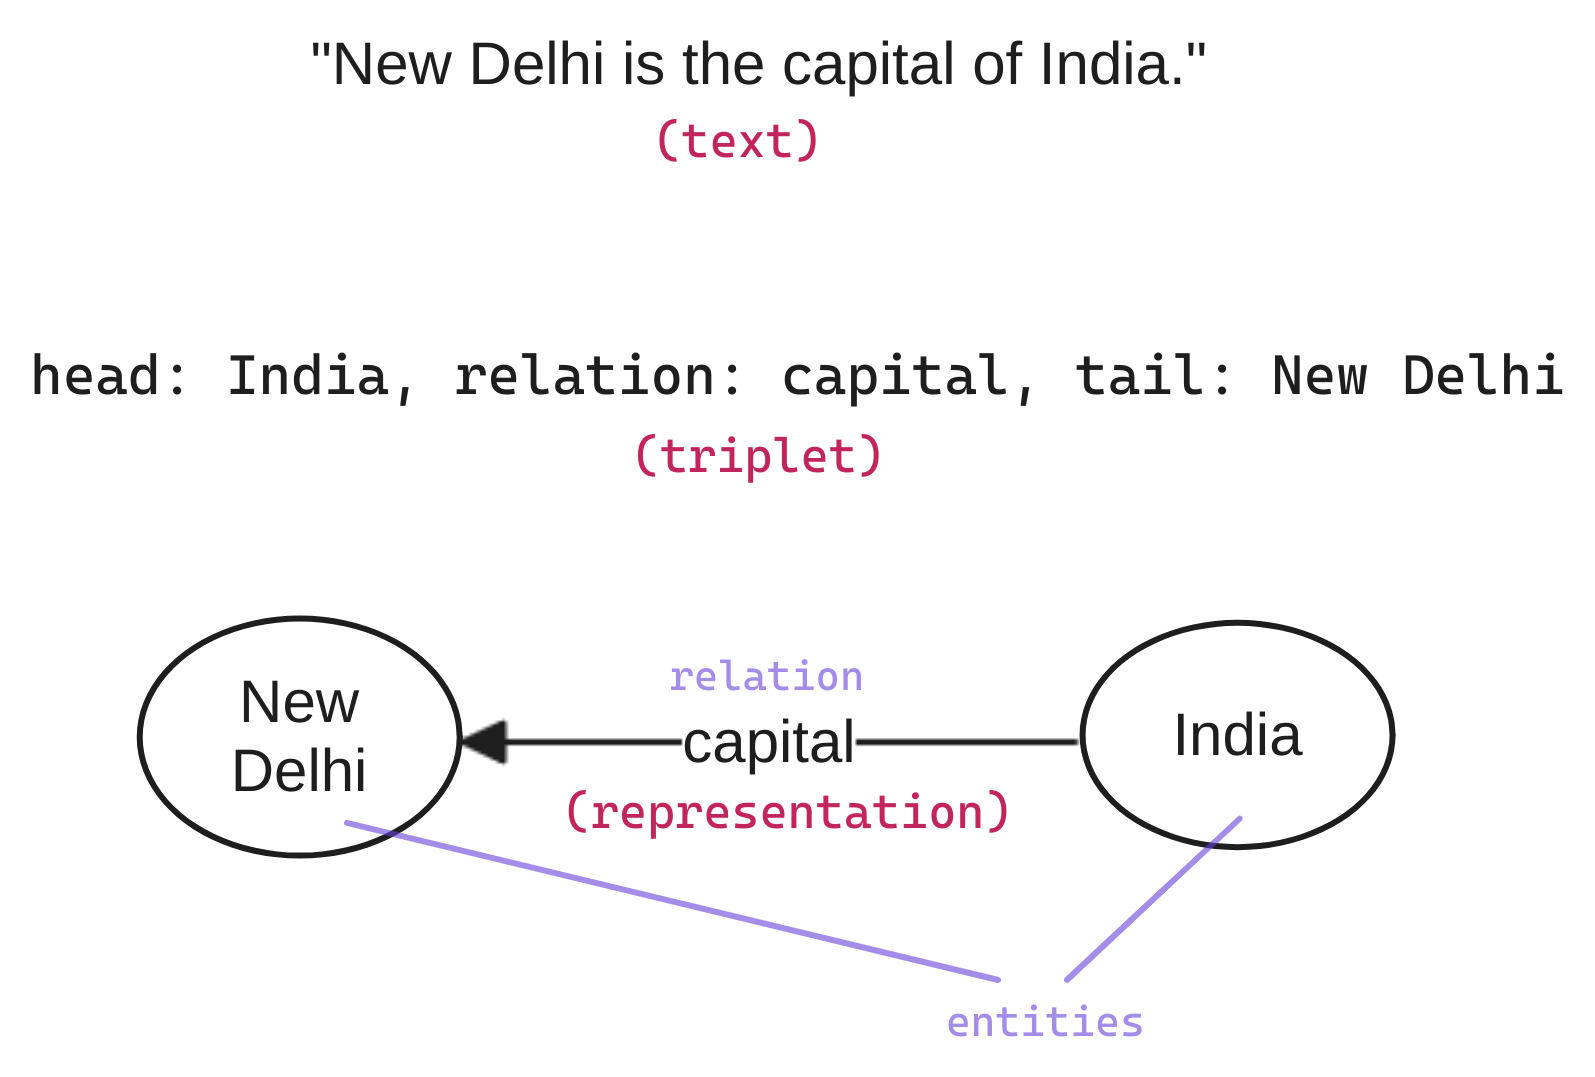
\includegraphics[width=0.9\textwidth]{attachments/triplets.png}
        \caption{Building a triplet}
        \label{fig:triplet}
\end{figure}
\end{frame}

\begin{frame}{Paper Review \cite{paper}}
    \begin{itemize}
        \item The problem: representation of KG embeddings, no specific models
        \item Existing Translation-based and Semantic matching models
        \item considered only KG triplets, suffer from structure sparsity
        \item Text-enhanced representation: using CNNs and LSTMs
    \end{itemize}
\end{frame}

\begin{frame}{Paper Review \cite{paper} (cont.)}
    Proposed Method (Teger):
    \begin{itemize}
        \item Triplet Embedding: $f (h, r, t) = -||h + r - t||^2$
        \item Auxiliary text encoding: Text-graph construction: $G = \{V, E\}$
        \item Knowledge Graph Fusion: integrating auxiliary embeddings and triplet using gating vector  = CONVOLUTION!
        \item End-to-end training = Loss = margin between incorrect (samples) and correct triplets
    \end{itemize}
\end{frame}

\begin{frame}{Progress with KG creation}
    Challenges with models we tested:
    \begin{itemize}
        \item Mistral-7B: Computationally expensive
        \item FRED: The links were ambiguous
        \item REBEL: Had a token limit of 1024 tokens (roughly 730 words)
    \end{itemize}
    Break down corpus into parts? Some information will be lost.
    Solution (or rather work-around) would be to continue working with end-to-end models but with smaller input and parallely check out separate models for NER and RC. 
\end{frame}

\begin{frame}{Visualisation}
    \begin{itemize}
        \item NetworkX and PyVis, don't support heterogenous graphs
        \item Graphviz, Neo4j and Pytorch Geometric support heterogenous graphs
        \item Neoj4 is interactive
    \end{itemize}
\end{frame}

\begin{frame}{Next Steps}
    \begin{itemize}
        \item Test separate models for NER and RC instead of an end-to-end model 
        \item Choose best combination(s) from multiple NER and RC models
        \item Link Prediction models and applying GNNs to KG processing tasks
    \end{itemize}
\end{frame}




\begin{frame}{References}
    \printbibliography
\end{frame}

\end{document}

% example of a triplet